\begin{figure}[ht]
\centering
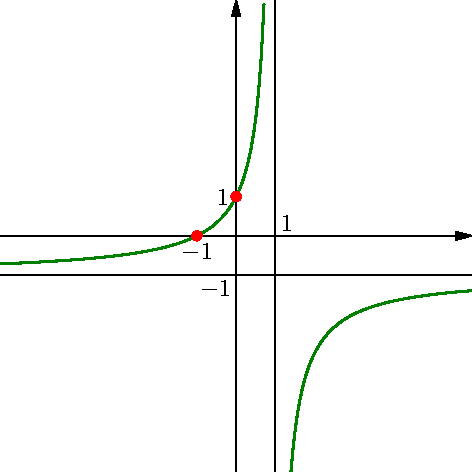
\includegraphics[width=5cm]{Chomog_1.pdf}
\caption{Graphe de $\varphi$}
\label{fig: Chomog_1}
\end{figure}

\begin{enumerate}
 \item Pour former le graphe de $\varphi$ (Figure \ref{fig: Chomog_1}), il est inutile de dériver la fonction. L'écriture
\begin{displaymath}
 \varphi(z) = \frac{1+z}{1-z} = \frac{2+z-1}{1-z} = -1 + \frac{2}{1-z}
\end{displaymath}
met en évidence les asymptotes et le fait que le graphe est une hyperbole. Pour placer les branches, on considère $\varphi(0)=1$.

\item Pour montrer que la fonction $f$ est une bijection de $\C-\{-1\}$ dans $\C-\{3\}$, on considère l'équation 
\[
 \frac{3z-5}{z+1} = u \text{ d'inconnue $z$ et de paramètre } u\in \C, u \neq 3.
\]
Cette équation admet une unique solution $\frac{u+5}{3-u}$ ce qui montre que tout $u\in\C$, $u\neq 3$ admet un unique antécédent par $f$. L'expression de la solution nous donne cet antécédent et donc une expression de la bijection réciproque.\newline
Par définition d'une implication (contraposition):
\[
 \left( z\notin \R \Rightarrow f(z)\notin \R \right) \Leftrightarrow \left( f(z) \in \R \Rightarrow z \in \R\right). 
\]
Cette deuxième implication résulte de 
\[
 f(z) \in \R \Rightarrow z = \frac{3f(z) - 5}{f(z) + 1} \in  \R.
\]


\item Tranformons la relation proposée : on utilise l'identité donnant $|a + b|^2$, on rassemble les termes, on divise par $1-k^2\neq0$:
\begin{multline*}
 |z - a|^2 = k^2|z-b|^2
\Leftrightarrow (1-k^2)|z|^2 -2\Re(a-k^2b)\overline{z} + |a|^2-k^2|b|^2 =0 \\
\Leftrightarrow |z|^2 -2\Re\frac{a-k^2b}{1-k^2}\overline{z} = \frac{-|a|^2+k^2|b|^2}{1-k^2}\\
\Leftrightarrow \left\vert z- \frac{a-k^2b}{1-k^2} \right \vert^2 = \frac{-|a|^2+k^2|b|^2}{1-k^2} + \frac{|a-k^2b|^2}{(1-k^2)^2}
\end{multline*}
Notons $T$ le membre de droite de la dernière relation :
\begin{displaymath}
 T = \frac{1}{(1-k^2)^2}\left( k^2|a|^2+k^2|b|^2 -2k^2\Re(a\overline{b})\right)
= \frac{k^2}{(1-k^2)^2}|a-b|^2 
\end{displaymath}
On en déduit le $u$ et le $R$ demandés par l'énoncé :
\[
 u = \frac{1}{1-k^2}(a-k^2b), \hspace{1cm} R = \frac{k}{1-k^2}|a-b|. 
\]
Il apparait alors clairement que l'ensemble des points dont l'affixe vérifie cette relation est un cercle de centre le point d'affixe $u$ et de rayon $R$.

\item La recherche des points fixes de $f$ conduit à l'équation du second degré
\begin{displaymath}
 z^2 -2z +5 =0
\end{displaymath}
Son discriminant est $\Delta=-16=(4i)^2$. On en déduit $z_1 = 1 + 2i$, $z_2 = 1-2i$.

\item Travaillons d'abord sur $f(z)-z_1$ en écrivant $z_1=f(z_1)$ et en réduisant au même dénominateur. On obtient
\begin{displaymath}
 f(z)-z_1 = f(z)-f(z_1) = \frac{3z-5}{z+1} -\frac{3z_1-5}{z_1+1} = \frac{8(z-z_1)}{(z+1)(z_1+1)}
\end{displaymath}
Le calcul est analogue pour $z_2$. On en déduit :
\begin{displaymath}
 \frac{f(z)-z_1}{f(z)-z_2} = \frac{(z_2+1)(z-z_1)}{(z_1+1)(z-z_2)} = \left( \frac{1-i}{1+i}\right) \frac{z-z_1}{z-z_2}
\end{displaymath}

\item \begin{enumerate}
\item L'ensemble des points est un cercle d'après la question 3.
\item Le centre du cercle est le point d'affixe $u$ de la question 3. Ici cela devient :
\begin{displaymath}
 u = \frac{1}{1-k^2}(z_1 -k^2z_2) = \frac{1}{1-k^2}(1-k^2 +2i(1+k^2)) = 1 + 2\varphi(k^2)i
\end{displaymath}
On cherche les points d'intersections du cercle avec la droite $(Z_1Z_2)$ sous la forme
\begin{displaymath}
 z= z_1 + \lambda (z_2-z_1) \text{ avec } \lambda \in \R
\end{displaymath}
La condition d'intersection s'écrit alors simplement en $\lambda$ : $\left \vert \frac{\lambda}{\lambda -1}\right \vert = k$.
Cela conduit à deux équations du premier degré selon que l'on prenne l'intérieur de la valeur absolue égal à $k$ ou à $-k$.
\begin{itemize}
 \item Pour $k$, on obtient $\lambda=-\frac{k}{1-k}$ et un point d'intersection d'affixe $1+2i\varphi(k)$.
 \item Pour $-k$, on obtient $\lambda= \frac{k}{1+k}$ et un point d'intersection d'affixe $1+2i\varphi(-k)$.
On peut remarquer que $\varphi(-k)$ est l'inverse de $\varphi(k)$.
\end{itemize}
\end{enumerate}

\begin{figure}[!h]
\centering
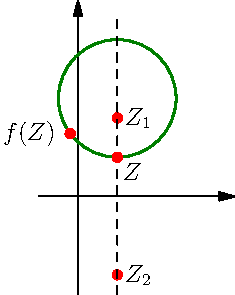
\includegraphics[width=4cm]{Chomog_2.pdf}
\caption{Cercle de $\mathcal C_\frac{1}{3}$}
\label{fig:Chomog_2}
\end{figure}

\item \begin{enumerate}
\item On a vu que 
\begin{displaymath}
 \left \vert \frac{f(z)-z_1}{f(z)-z_1}\right\vert = \left\vert \frac{1-i}{1+i} \frac{z-z_1}{z-z_2}\right\vert 
= \left\vert \frac{z-z_1}{z-z_2}\right\vert 
\end{displaymath}
Si on note $f^n$ la composée de $f$ avec elle même $n$ fois, on a alors:
\begin{displaymath}
 \left \vert \frac{f^n(z)-z_1}{f^n(z)-z_1}\right\vert = \left \vert \frac{f^{n-1}(z)-z_1}{f^{n-1}(z)-z_1}\right\vert 
= \cdots = \left \vert \frac{z-z_1}{z-z_1}\right\vert
\end{displaymath}
Ce qui signifie que tous les points sont sur $\mathcal C_k$ avec $k = \left \vert \frac{z-z_1}{z-z_1}\right\vert$.


\item Pour $z=1+i$, on trouve $k=\vert \frac{-i}{3i}\vert=\frac{1}{3}$, $\varphi(\frac{1}{3})=2$.\newline
On en déduit que les points d'intersections avec $(Z_1Z_2)$ ont pour coordonnées $(1,1)$ et $(1,4)$. Le centre du cercle $\mathcal{C}_{\frac{1}{3}}$ (Figure \ref{fig:Chomog_2})  est en $(1,\frac{5}{2})$ et le rayon est $\frac{3}{2}$. De plus $f(z)=\frac{-1+8i}{5}$.
\end{enumerate}
\end{enumerate}
